\documentclass[12pt]{article}
\usepackage{graphicx}
\usepackage{float}
\usepackage{amsmath}
\title{Experiment 2: 4-to-2 Encoder, Priority Encoder and 8-to-3 Encoder}
\author{Annirudh K P Roll Number 210070009}

\begin{document}

\maketitle

\section{Overview of the experiment}
\paragraph{}
In this experiment, we started working on more designs using structure modelling on VHDL. The problem statement of this experiment is to design the 4 to 2 encoder, Priority Encoder and the 8 to 3 encoder, and then describe them in VHDL using structural modelling. The objective of this experiment was to understand the Quartus Design Flow, and give us hands on experience over different technical glitches/problems we may face in this piece of software which has been made unwantedly hard.

\section{Experimental Set-up}

\subsection{Design Requirements}
\subsubsection{4 to 2 Encoder}
A 4 to 2 encoder has 5 inputs : A, B, C, D and EN and 2 outputs: Y1, Y0. The truth table is shown below.

\begin{figure}[H]
\centering
  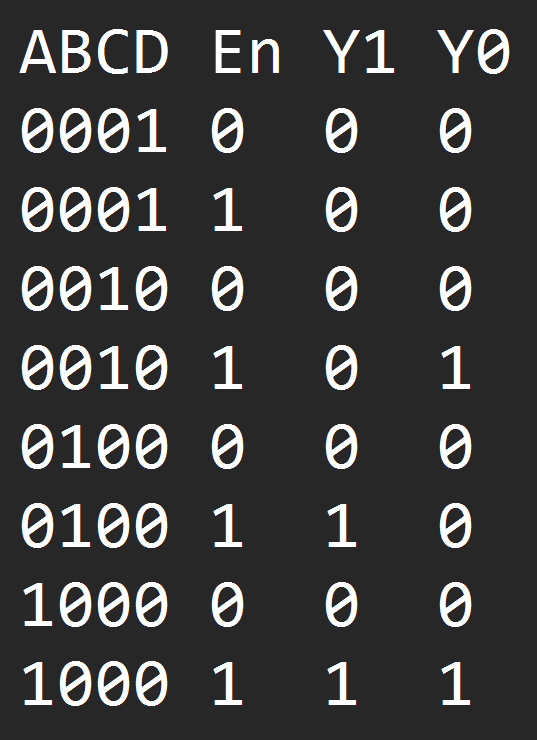
\includegraphics[scale=0.3]{Images/4to2TT.png}
  \caption{4 to 2 Encoder Truth Table}
\end{figure}

\subsubsection{4 to 2 Priority Encoder}
A 4 to 2 priority encoder was required to be designed which has 4 inputs : A, B, C and D and 3 outputs: Y1, Y0 and V. The truth table is shown below.

\begin{figure}[H]
\centering
  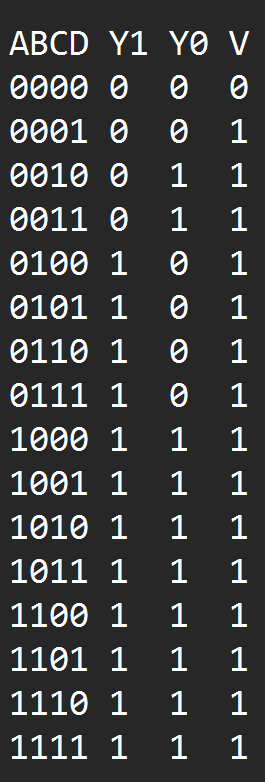
\includegraphics[scale=0.3]{Images/4to2PriorityTT.png}
  \caption{4 to 2 Priority Encoder Truth Table}
\end{figure}

\subsubsection{8 to 3 Encoder}
A 8 to 3 encoder was required to be designed which has 9 inputs : Y7, Y6, Y5, Y4, Y3, Y2, Y1, Y0, E and 3 outputs: A2, A1 and A0. The truth table is shown below.

\begin{figure}[H]
\centering
  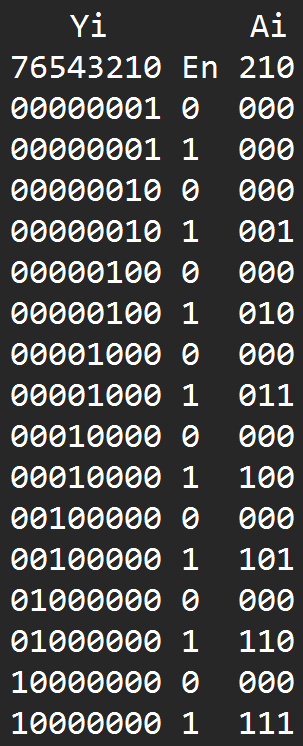
\includegraphics[scale=0.3]{Images/8to3TT.png}
  \caption{8 to 3 Encoder Truth Table}
\end{figure}

\subsection{Design Schematics}
The following design schematics are shown. For the 8 to 3 Encoder design we were restricted only use the OR Gates and the 4 to 2 Encoders we had designed in the earlier part. 

\begin{figure}[H]
\centering
  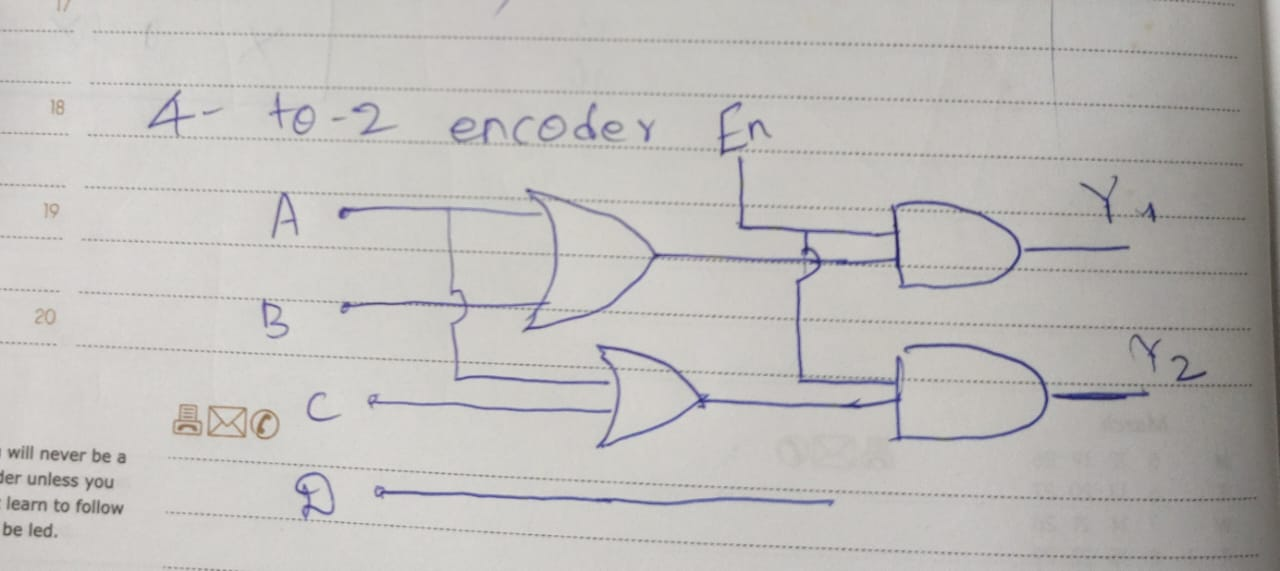
\includegraphics[scale=0.3]{Images/4to2ENCODER_DESIGN.png}
  \caption{4 to 2 Encoder Design}
\end{figure}

\begin{figure}[H]
\centering
  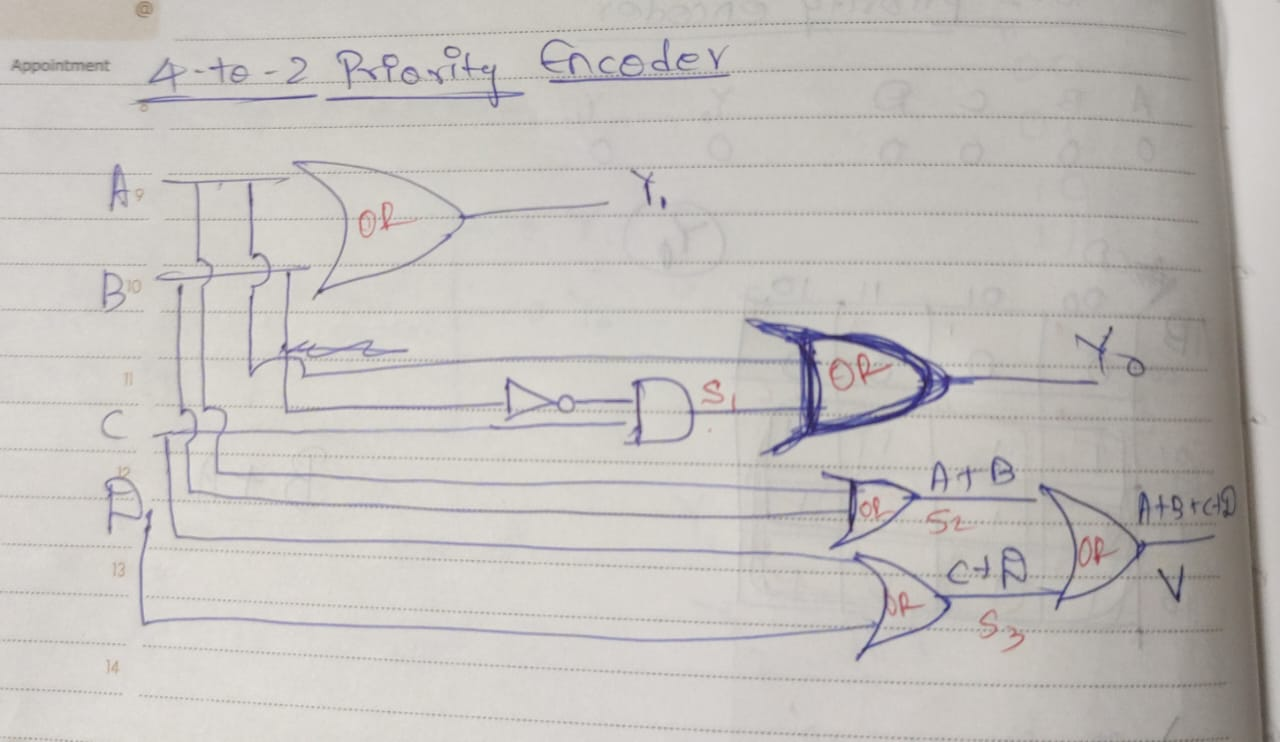
\includegraphics[scale=0.3]{Images/PriorityEnc_DESIGN.png}
  \caption{4 to 2 Priority Encoder Design}
\end{figure}

\begin{figure}[H]
\centering
  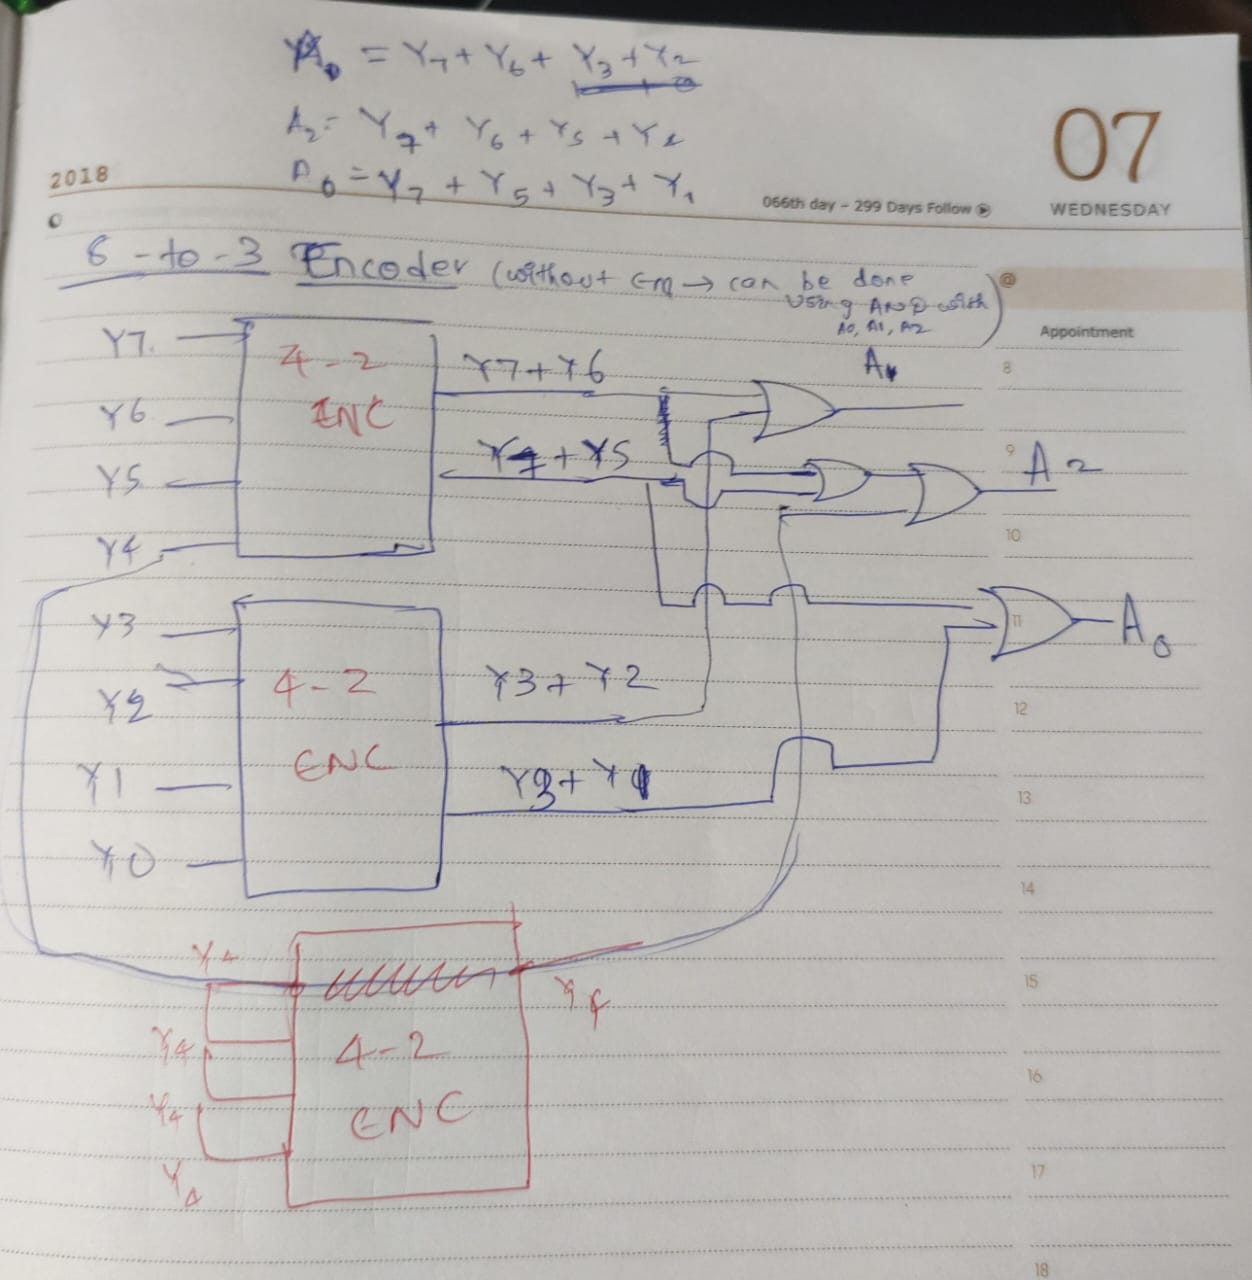
\includegraphics[scale=0.3]{Images/8to3ENCODER_DESIGN.jpeg}
  \caption{8 to 3 Encoder Design}
\end{figure}

\begin{figure}[H]
\centering
  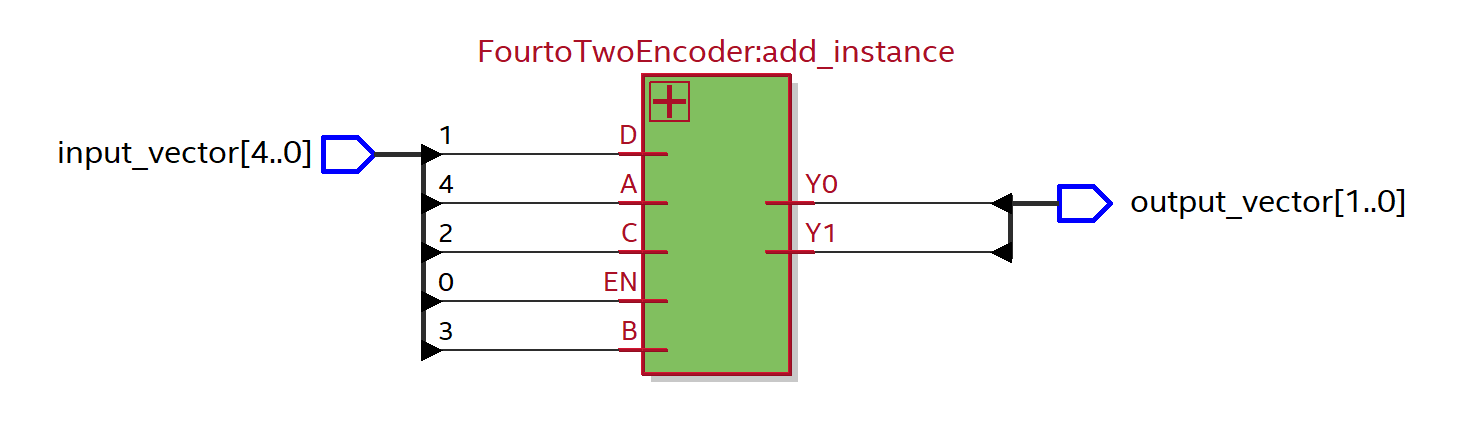
\includegraphics[scale=0.3]{Images/4to2ENCODER_RTLVIEWER.png}
  \caption{4 to 2 Encoder RTL Design}
\end{figure}

\begin{figure}[H]
\centering
  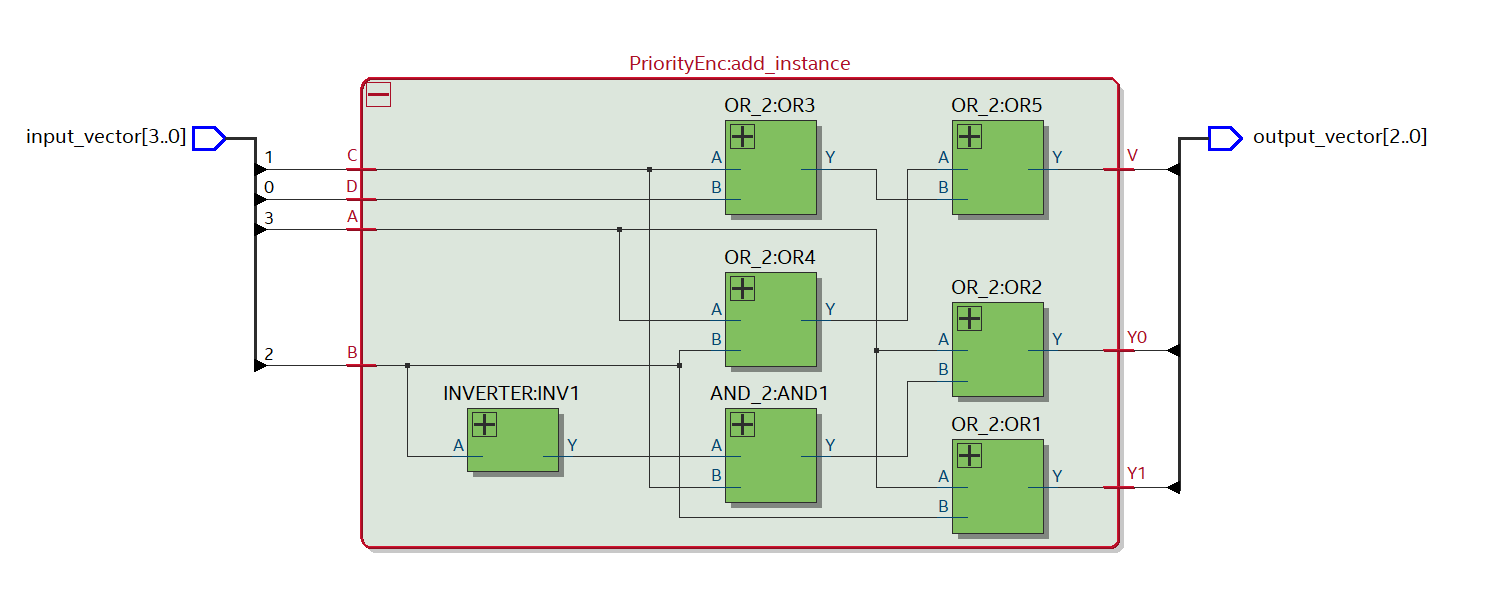
\includegraphics[scale=0.3]{Images/PriorityEnc_RTLVIEWER.png}
  \caption{4 to 2 Priority Encoder RTL Design}
\end{figure}

\begin{figure}[H]
\centering
  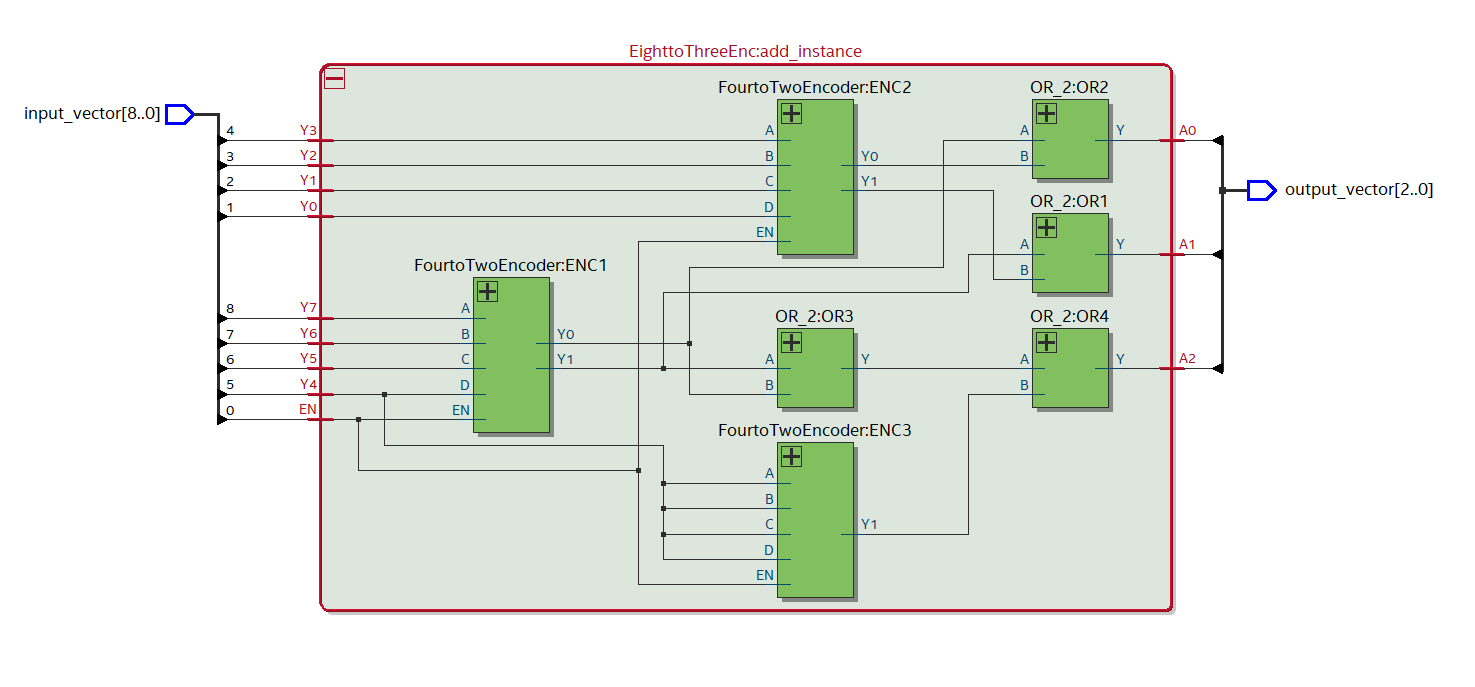
\includegraphics[scale=0.3]{Images/8to3ENCODER_RTLVIEWER.png}
  \caption{8 to 3 Encoder RTL Design}
\end{figure}

\subsection{Description of Components}
\subsubsection{4 to 2 Encoder}
\begin{verbatim}
library ieee;
use ieee.std_logic_1164.all;
library work;
use work.Gates.all;

entity FourtoTwoEncoder  is
  port (A, B, C, D, EN: in std_logic; Y1, Y0: out std_logic);
end entity FourtoTwoEncoder;

architecture Logic of FourtoTwoEncoder is
  signal S1, S2 : std_logic;
begin
  -- component instances
  OR1: OR_2 port map (A => A, B => B, Y => S1);
  OR2: OR_2 port map (A => A, B => C, Y => S2);
  AND1: AND_2 port map (A => S1, B => EN, Y => Y1);
  AND2: AND_2 port map (A => S2, B => EN, Y => Y0);
end Logic;
\end{verbatim}

\subsubsection{4 to 2 Priority Encoder}
\begin{verbatim}
library ieee;
use ieee.std_logic_1164.all;
library work;
use work.Gates.all;

entity PriorityEnc  is
  port (A, B, C, D: in std_logic; Y1, Y0, V: out std_logic);
end entity PriorityEnc;

architecture Logic of PriorityEnc is
  signal B_BAR, S1, S2, S3 : std_logic;
begin
  -- component instances
  OR1: OR_2 port map (A => A, B => B, Y => Y1);
  INV1: INVERTER port map (A => B, Y => B_BAR);
  AND1: AND_2 port map (A => B_BAR, B => C, Y => S1);
  OR2: OR_2 port map (A => A, B => S1, Y => Y0);
  OR3: OR_2 port map (A => C, B => D, Y => S2);
  OR4: OR_2 port map (A => A, B => B, Y => S3);
  OR5: OR_2 port map (A => S3, B => S2, Y => V);
end Logic;
\end{verbatim}

\subsubsection{8 to 3 Encoder}
\begin{verbatim}
library ieee;
use ieee.std_logic_1164.all;
library work;
use work.Gates.all;

entity FourtoTwoEncoder  is
  port (A, B, C, D, EN: in std_logic; Y1, Y0: out std_logic);
end entity FourtoTwoEncoder;

architecture Logic of FourtoTwoEncoder is
  signal S1, S2 : std_logic;
begin
  -- component instances
  OR1: OR_2 port map (A => A, B => B, Y => S1);
  OR2: OR_2 port map (A => A, B => C, Y => S2);
  AND1: AND_2 port map (A => S1, B => EN, Y => Y1);
  AND2: AND_2 port map (A => S2, B => EN, Y => Y0);
end Logic;

library ieee;
use ieee.std_logic_1164.all;
library work;
use work.Gates.all;

entity EighttoThreeEnc  is
  port (Y7, Y6, Y5, Y4, Y3, Y2, Y1, Y0, EN: in std_logic; 
  			 A2, A1, A0: out std_logic);
end entity EighttoThreeEnc;

architecture Logic1 of EighttoThreeEnc is
  signal S1, S2, S3, S4, S5, S6, S7 : std_logic;
  component FourtoTwoEncoder is
		port (A, B, C, D, EN: in std_logic; Y1, Y0: out std_logic);
	end component FourtoTwoEncoder;
begin
  -- component instances
  ENC1: FourtoTwoEncoder port map (A => Y7, B => Y6, C => Y5, D => Y4, 
  			 EN => EN, Y1 => S1, Y0 => S2);
  ENC2: FourtoTwoEncoder port map (A => Y3, B => Y2, C => Y1, D => Y0,
  			 EN => EN, Y1 => S3, Y0 => S4);
  ENC3: FourtoTwoEncoder port map (A => Y4, B => Y4, C => Y4, D => Y4, 
  			 EN => EN, Y1 => S6, Y0 => S7);
  OR1: OR_2 port map (A => S1, B => S3, Y => A1);
  OR2: OR_2 port map (A => S2, B => S4, Y => A0);
  OR3: OR_2 port map (A => S1, B => S2, Y => S5);
  OR4: OR_2 port map (A => S5, B => S6, Y => A2);
end Logic1;
\end{verbatim}

\section{Observations}
 
We get RTL simulation waveforms for corresponding to input and output which is given below and it shows required results.

\begin{figure}[H]
\centering
  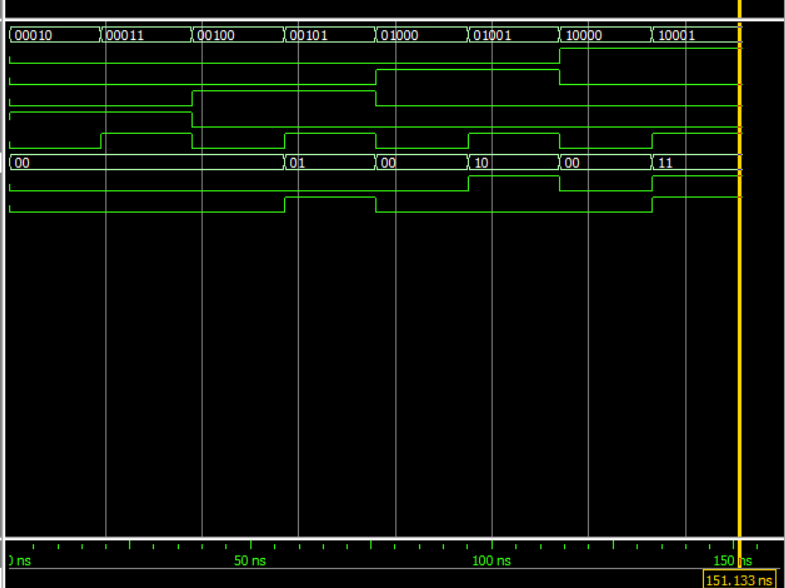
\includegraphics[scale=0.45]{Images/4to2ENCODER_RTLSIMULATION.png}
  \caption{4 to 2 Encoder RTL Simulation Waveform}
\end{figure}

\begin{figure}[H]
\centering
  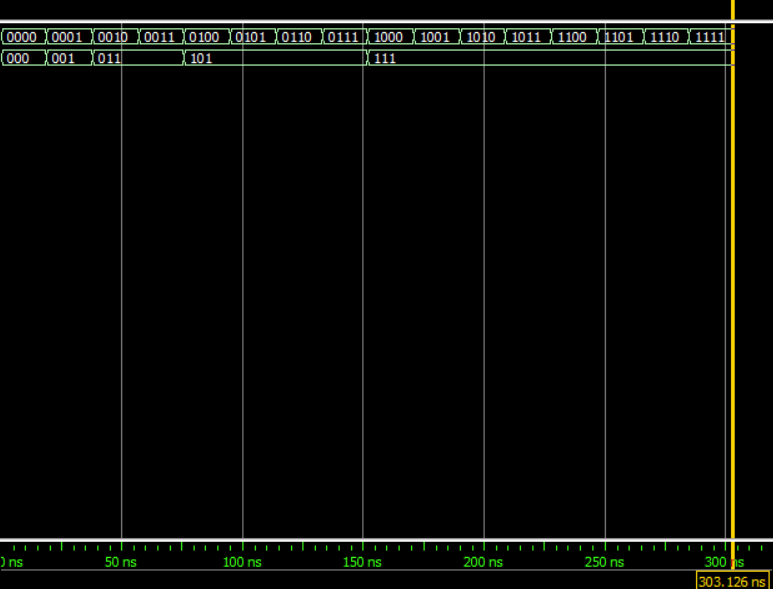
\includegraphics[scale=0.45]{Images/PriorityEnc_RTLSIMULATION.png}
  \caption{4 to 2 Priority Encoder RTL Simulation Waveform}
\end{figure}

\begin{figure}[H]
\centering
  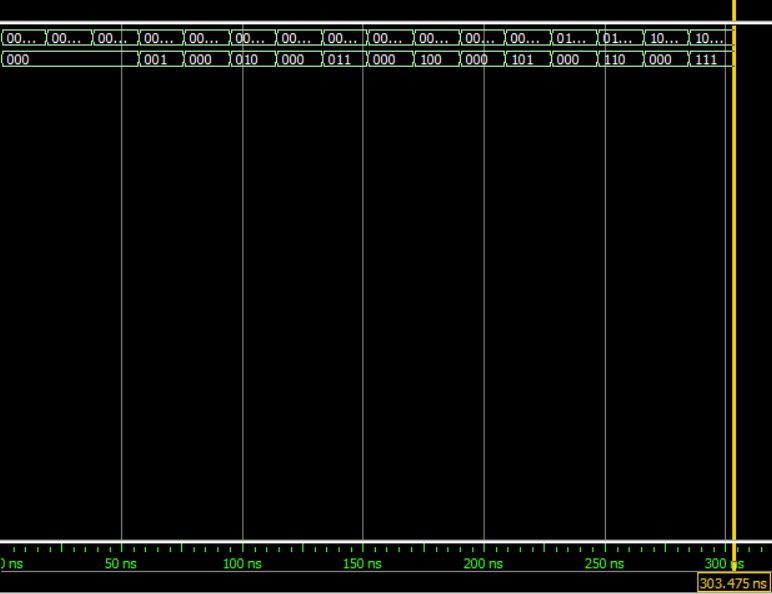
\includegraphics[scale=0.45]{Images/8to3ENCODER_RTLSIMULATION.png}
  \caption{8 to 3 Encoder RTL Simulation Waveform}
\end{figure}

\end{document}